\section{Additional Local-Palette and Candidate-Law Diagnostics}
\IfFileExists{figures/local-degree-heterogeneity.pdf}{
\begin{figure}[ht]\centering
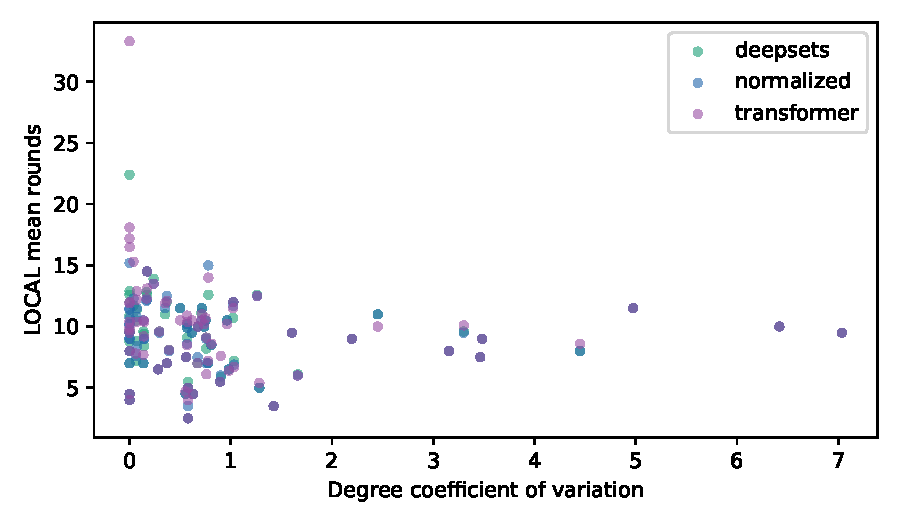
\includegraphics[width=.78\linewidth]{figures/local-degree-heterogeneity.pdf}
\caption{LOCAL mean rounds by degree heterogeneity. Points share graph
identities across architectures. This association alone is not a causal effect.}
\end{figure}}{}
\IfFileExists{figures/candidate-laws-k201.pdf}{
\begin{figure}[ht]\centering
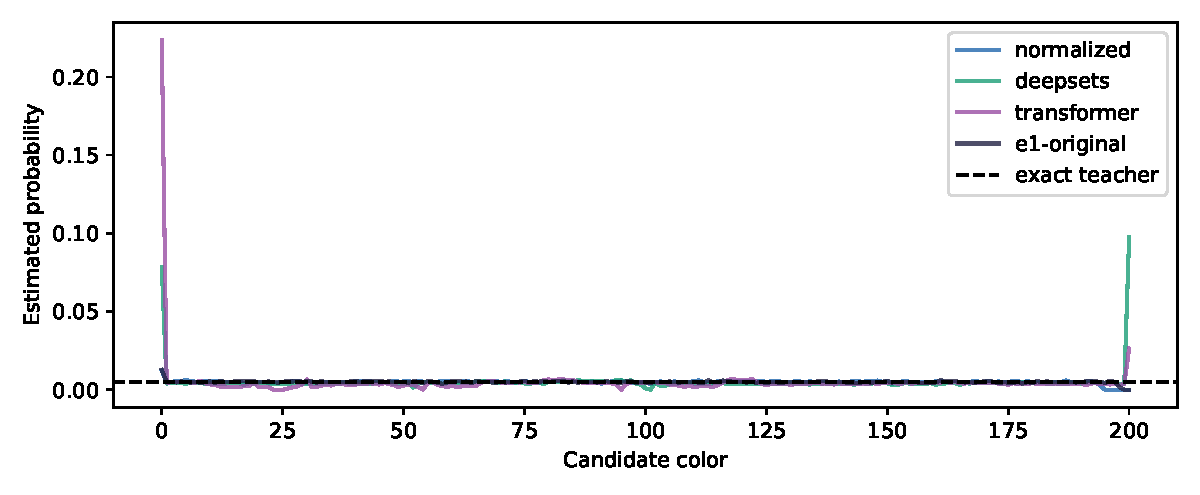
\includegraphics[width=.9\linewidth]{figures/candidate-laws-k201.pdf}
\caption{Estimated candidate probabilities in the same all-free $K=201$ state,
seed 41000 for each new architecture. The teacher line is analytically uniform.
All five replicas and the separately labeled original E1 cohort are in CSV.}
\end{figure}}{}
\IfFileExists{figures/diversity-and-progress.pdf}{
\begin{figure}[ht]\centering
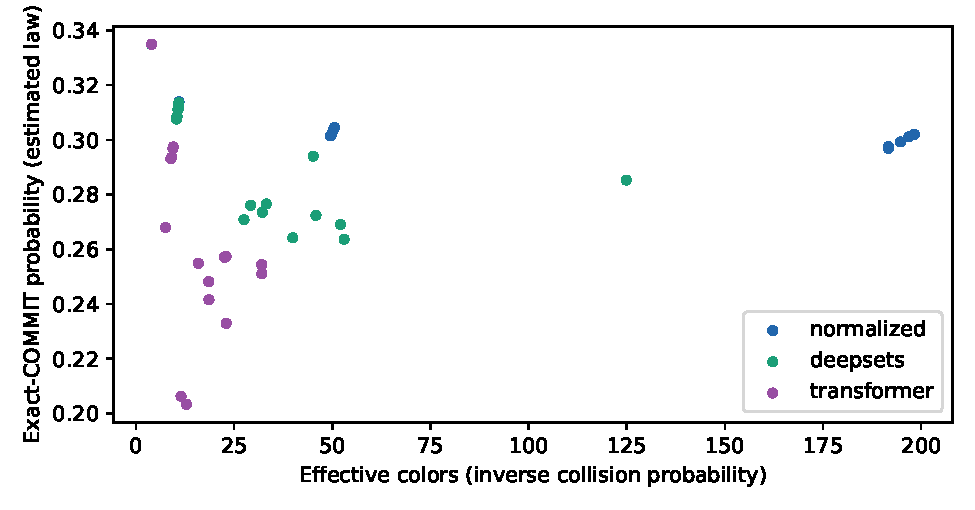
\includegraphics[width=.8\linewidth]{figures/diversity-and-progress.pdf}
\caption{Candidate diversity and predicted exact-COMMIT probability on shared
all-free clique states. Predictions use estimated laws and fixed participation
probability $1/2$, not a universal guarantee from the diversity metric.}
\end{figure}}{}
\IfFileExists{figures/candidate-mixture-intervention.pdf}{
\begin{figure}[ht]\centering
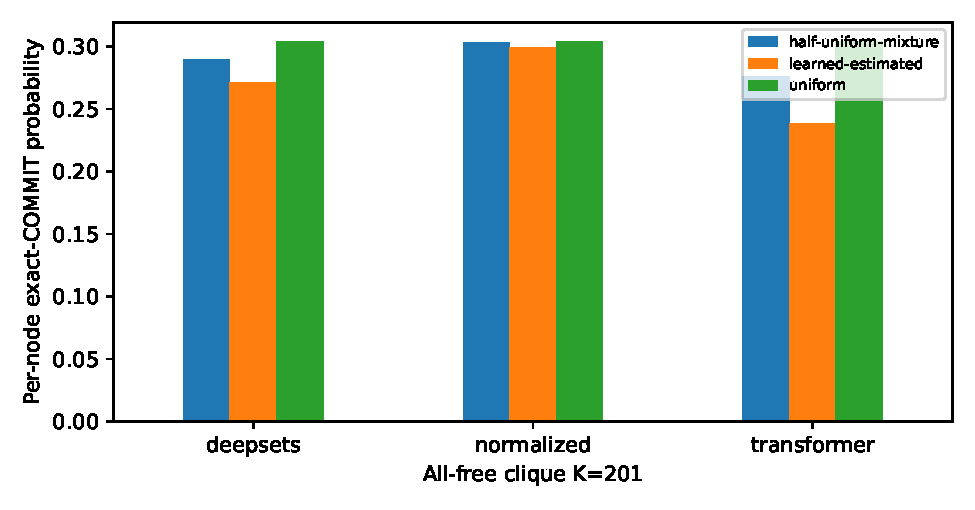
\includegraphics[width=.8\linewidth]{figures/candidate-mixture-intervention.pdf}
\caption{Controlled candidate-law substitution in the all-free $K=201$ clique:
estimated learned law, uniform law, and their 50:50 mixture. COMMIT is exact and
participation is fixed at $1/2$ for this intervention.}
\end{figure}}{}
\IfFileExists{figures/heterogeneous-state-progress.pdf}{
\begin{figure}[ht]\centering
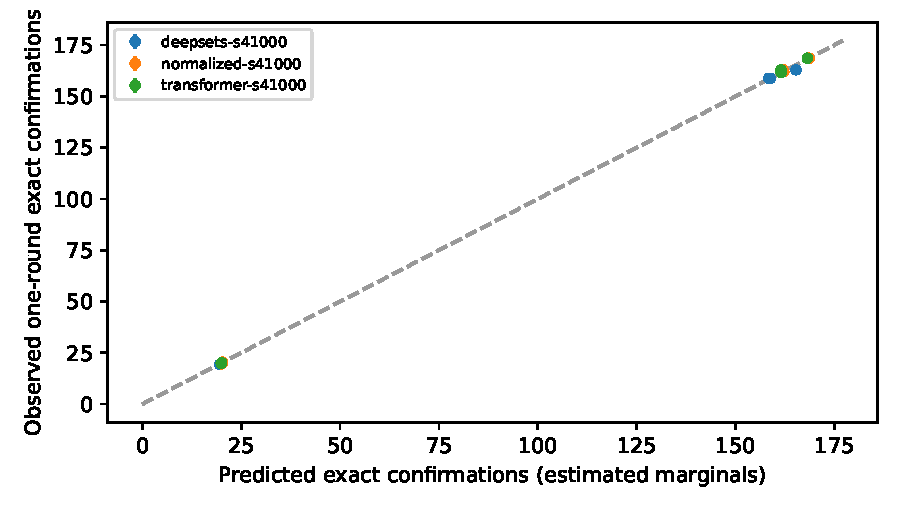
\includegraphics[width=.8\linewidth]{figures/heterogeneous-state-progress.pdf}
\caption{Six frozen heterogeneous LOCAL states, three new seed-41000 policies.
Predictions from independently estimated candidate/participation marginals are
compared with 256 fresh one-round exact-COMMIT observations per context.
Error bars show 1.96 Monte Carlo standard errors for the observations;
they do not include uncertainty in the predicted marginals.}
\end{figure}}{}
